\documentclass[reprint,superscriptaddress, amsmath,amssymb, aps, pra, longbibliography]{revtex4-1}
\usepackage{amsmath}
\usepackage{sansmath}

\usepackage{tikz}
\usetikzlibrary{calc}
\usepackage{xcolor}

\definecolor{DarkBlue}{rgb}{0.1,0.1,0.5}
\definecolor{DarkRed}{rgb}{0.75,0.,0.}
%\definecolor{tcbcolback}{rgb}{0.953,0.953,0.953} % poster
\definecolor{tcbcolback}{rgb}{1.0,1.0,1.0}

\usepackage[psfixbb,graphics,tightpage,active]{preview}
\PreviewEnvironment{tikzpicture}
\sansmath

\begin{document}

\newcommand{\xangle}{7}
\newcommand{\yangle}{137.5}
\newcommand{\zangle}{90}

\newcommand{\xlength}{1}
\newcommand{\ylength}{0.5}
\newcommand{\zlength}{1}

\newcommand{\R}{2.5}

\pgfmathsetmacro{\xx}{\xlength*cos(\xangle)}
\pgfmathsetmacro{\xy}{\xlength*sin(\xangle)}
\pgfmathsetmacro{\yx}{\ylength*cos(\yangle)}
\pgfmathsetmacro{\yy}{\ylength*sin(\yangle)}
\pgfmathsetmacro{\zx}{\zlength*cos(\zangle)}
\pgfmathsetmacro{\zy}{\zlength*sin(\zangle)}

\tikzset{
  A/.pic = {
    \node[inner sep = 0pt, anchor = south] at (0,0) {%
      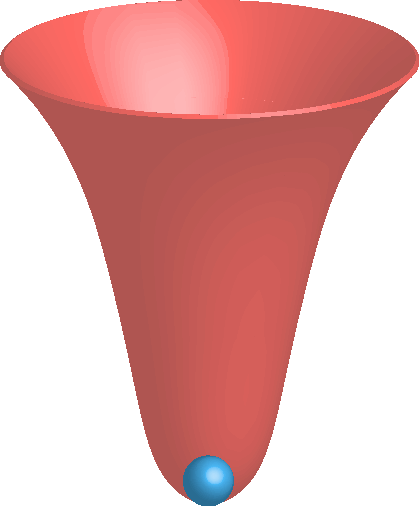
\includegraphics[width=1.3cm]{trapped_atom_A}
    };
    \node[fill = tcbcolback, inner sep=0pt, rounded corners, fill opacity = 0.9]
    at (-8pt, 1.8cm) {\color{DarkRed}$V_{+}(\theta)$};
    \node[inner sep=1pt, anchor = north west]
    at (0pt, -1pt) {\color{DarkRed}$\Psi_{\!+}$};
  }
}
\tikzset{
  B/.pic = {
    \node[inner sep = 0pt, anchor = south] at (0,0) {%
      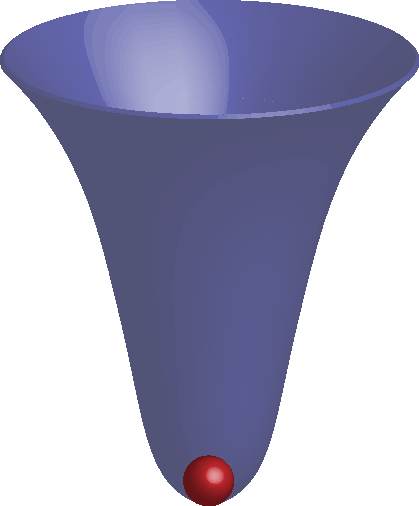
\includegraphics[width=1.3cm]{trapped_atom_B}
    };
    \node[fill = tcbcolback, inner sep=0pt, rounded corners, fill opacity = 0.9]
    at (8pt, 1.8cm) {\color{DarkBlue}$V_{-}(\theta)$};
    \node[inner sep=1pt, anchor = north west]
    at (0pt, -1pt) {\color{DarkBlue}$\Psi_{\!-}$};
  }
}


\begin{tikzpicture}
[   x={(\xx cm,\xy cm)},
    y={(\yx cm,\yy cm)},
    z={(\zx cm,\zy cm)},
    font=\small
]

  \fill[gray!30] (0,0,0) circle (\R);
  \draw[dashed, line width = 1pt] (0,0,0) circle (\R);
  \fill[color = black!70] (0,0,0) circle (1pt);
  \draw[->, line width = 1pt, color = black!70]
    (0,0,0) -- node[midway, below] {$R$} (0:\R);
  \path (120:\R) pic {A};
  \path (-120:\R) pic {B};
  \draw[->, line width = 2pt, color = DarkRed]
    (120:\R) arc (120:150:\R)
    node[pos=0, left=4pt] {\color{black}\small $\Omega + \omega(t)$};
  \draw[->, line width = 2pt, color = DarkBlue]
    (-120:\R) arc (-120:-150:\R)
    node[pos=1.0, below] {\color{black}\small $\Omega - \omega(t)$};


\end{tikzpicture}

\end{document}
